% =============================================
% File: chapters/methodology.tex
% Chương 3: Phương pháp thực hiện
% =============================================

\chapter{PHƯƠNG PHÁP THỰC HIỆN}
\label{chap:phuongphap}

Chương # trình bày toàn bộ quy trình và phương pháp cụ thể được áp dụng
trong đề tài, gồm hai hướng song song: (1)~\textbf{hướng điều khiển cổ điển}
— thu thập dữ liệu, nhận dạng hàm truyền động cơ, tối ưu tham số bộ điều
khiển tầng bằng giải thuật di truyền, xây dựng mạng ANN dự đoán tham số
thích nghi, và triển khai trên vi điều khiển ESP32; (2)~\textbf{hướng học
tăng cường} — xây dựng môi trường mô phỏng trong Isaac Lab, huấn luyện
chính sách điều khiển bằng thuật toán PPO và xuất trọng số để triển khai
thực tế.


% ==============================================
\section{Quy trình nghiên cứu tổng quan}
% ==============================================

Nghiên cứu được thực hiện theo hai hướng song song với 6 giai đoạn chính:

\begin{enumerate}
    \item \textbf{Giai đoạn 1 — Thu thập dữ liệu thực nghiệm:}
    Vận hành động cơ NF5475 theo giao thức kích thích bậc thang ở 5 mức PWM,
    đọc phản hồi vận tốc qua encoder 200~PPR và ghi log về máy tính qua
    cổng Serial (115\,200~baud).

    \item \textbf{Giai đoạn 2 — Nhận dạng hàm truyền:}
    Sử dụng MATLAB System Identification Toolbox (\texttt{tfest}) để xác định
    hàm truyền $G_{\text{vel}}(s)$ của động cơ; rời rạc hóa bằng phương pháp
    Tustin để phục vụ tối ưu GA.

    \item \textbf{Giai đoạn 3 — Tối ưu bộ điều khiển bằng GA:}
    Áp dụng giải thuật di truyền trên mô hình rời rạc để tìm bộ tham số tối
    ưu $(K_{pp}^*, K_{ip}^*, K_{dp}^*, K_{pv}^*, K_{iv}^*)$ cho bộ điều
    khiển cascade PID-vị trí + PI-vận tốc, tại nhiều mức setpoint.

    \item \textbf{Giai đoạn 4 — Xây dựng và huấn luyện ANN:}
    Từ bộ tham số GA tối ưu tại 9 setpoint vận tốc (250--2250~RPM),
    huấn luyện mạng ANN có khả năng dự đoán tham số PI thích nghi theo
    setpoint và sai số vận tốc hiện tại.

    \item \textbf{Giai đoạn 5 — Triển khai trên ESP32:}
    Cài đặt vòng điều khiển PI với tham số do ANN dự đoán lên vi điều khiển
    ESP32, thực nghiệm vận tốc và đánh giá đáp ứng hệ thống.

    \item \textbf{Giai đoạn 6 — Huấn luyện RL trong Isaac Lab:}
    Song song với hướng điều khiển cổ điển, xây dựng môi trường mô phỏng
    vật lý trong Isaac Lab và huấn luyện chính sách điều khiển chuyển động
    toàn thân bằng thuật toán PPO với curriculum 3 pha dựa trên hiệu suất.
    Sau huấn luyện, trọng số mạng Actor được xuất sang ONNX để triển khai
    thực tế.
\end{enumerate}

% ==============================================
\section{Mô tả hệ thống robot hai chân}
% ==============================================

\subsection{Kiến trúc tổng thể}

Bipedal Robot là robot hai chân có bánh xe, trong đó mỗi chân được dẫn động bởi cơ cấu song song 5 khâu (5-bar linkage). Bánh xe được gắn tại điểm cuối cùng của chân (end-effector), cho phép robot vừa di chuyển bằng bánh vừa thay đổi chiều cao thân thông qua việc điều khiển góc khớp.

\begin{figure}[H]
    \centering
    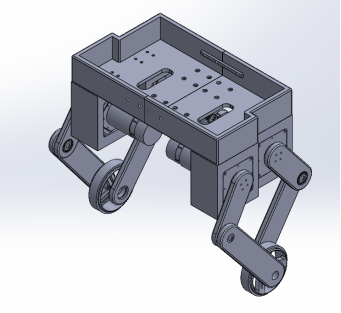
\includegraphics[width=0.45\textwidth]{figure/mohinhtongthe.png}
    \caption{Mô hình tổng thể Bipedal Robot}
    \label{fig:robot_overview}
\end{figure}

Robot gồm thân chính phía trên là khung chứa các linh kiện quan trong như mạch điện và cảm biến, hai cụm chân đối xứng qua mặt phẳng cắt giữa của khung và
1 bánh xe đặt tại điểm cuối mỗi chân. Mỗi cụm chân sử dụng hai động cơ NF5475
có encoder để điều khiển hai thanh chủ động; hai thanh bị động tạo thành chuỗi
động học kín, xác định vị trí điểm cuối $P$ để đặt trục bánh xe.

\begin{figure}[H]
    \centering
    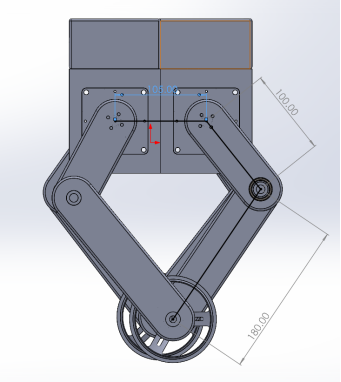
\includegraphics[width=0.45\textwidth]{figure/robotmohinh.png}
    \caption{Mô hình 3D Bipedal Robot}
    \label{fig:robot_3d}
\end{figure}

Hệ thống được chia thành ba cấp:
\begin{itemize}
    \item \textbf{Cấp cơ khí:} Khung nhôm định hình, hai cơ cấu 5-bar
    parallel, trục bánh xe.
    \item \textbf{Cấp dẫn động:} Bốn động cơ DC NF5475 (hai mỗi chân)
    kết hợp encoder quang học 200 PPR.
    \item \textbf{Cấp điều khiển:} Vi điều khiển ESP32 WROOM-32, mạch
    driver L298N, giao tiếp Serial/UART với máy tính.
\end{itemize}


\subsection{Cơ cấu 5-bar parallel}

Ký hiệu các thành phần cơ cấu được quy ước trong Bảng~\ref{tab:5bar_notation}.

\begin{table}[H]
    \centering
    \caption{Ký hiệu các thành phần cơ cấu 5-bar parallel}
    \label{tab:5bar_notation}
    \renewcommand{\arraystretch}{1.3}
    \begin{tabular}{|c|l|p{7cm}|}
    \hline
    \textbf{Ký hiệu} & \textbf{Tên} & \textbf{Mô tả} \\
    \hline
    $A_1,\,A_2$ & Khớp chủ động & Hai khớp quay cố định trên thân,
                  truyền động bởi động cơ NF5475 \\
    \hline
    $B_1,\,B_2$ & Khớp bị động & Nối giữa thanh chủ động và thanh bị động \\
    \hline
    $P$         & Điểm cuối     & Vị trí gắn cụm bánh xe \\
    \hline
    $d$         & Khoảng cách gốc & Khoảng cách $A_1A_2$ \\
    \hline
    $L_{act}$   & Thanh chủ động & Chiều dài $A_1B_1$ và $A_2B_2$ \\
    \hline
    $L_{pas}$   & Thanh bị động  & Chiều dài $B_1P$ và $B_2P$ \\
    \hline
    \end{tabular}
\end{table}

Thông số hình học của cơ cấu trong đề tài:

\begin{table}[H]
    \centering
    \caption{Thông số hình học cơ cấu 5-bar parallel}
    \label{tab:5bar_params}
    \renewcommand{\arraystretch}{1.3}
    \begin{tabular}{|l|c|c|}
    \hline
    \textbf{Thông số} & \textbf{Ký hiệu} & \textbf{Giá trị} \\
    \hline
    Khoảng cách hai khớp chủ động & $d = A_1A_2$ & 105 mm \\
    Chiều dài thanh chủ động      & $L_{act}$    & 100 mm \\
    Chiều dài thanh bị động       & $L_{pas}$    & 180 mm \\
    \hline
    \end{tabular}
\end{table}

Ưu điểm so với chân nối tiếp: (i)~độ cứng vững cao hơn do tải phân phối
trên hai thanh bị động, (ii)~khối lượng phần chuyển động nhỏ vì động cơ
đặt tại gốc cố định, (iii)~giảm số bậc tự do cần điều khiển xuống còn 2.


% ==============================================
\section{Thu thập dữ liệu và nhận dạng hàm truyền}
\label{sec:data_sysid}
% ==============================================

\subsection{Quy trình thu thập dữ liệu}

Dữ liệu đặc tính động cơ DC NF5475 được thu thập theo giao thức kích thích
bậc thang (\textit{step-input protocol}). Vi điều khiển ESP32 lần lượt áp
5 mức PWM cố định: $20\%$, $40\%$, $60\%$, $80\%$, $100\%$ (tương ứng 51,
102, 153, 204, 255 đơn vị 8-bit), mỗi mức duy trì trong \textbf{10 giây}.

Vận tốc tức thời được tính sau mỗi chu kỳ lấy mẫu $T_s = 0{,}01\;\text{s}$:
\begin{equation}
    v(k) = \frac{n_{\text{xung}}(k)}{200} \cdot \frac{60}{T_s}
    \qquad [\text{RPM}]
    \label{eq:vel_calc}
\end{equation}
trong đó $n_{\text{xung}}(k)$ là số xung encoder (200~PPR) tích lũy trong
khoảng $[kT_s,\,(k{+}1)T_s)$. Bộ ba $(t,\;v(k),\;u(k))$ được truyền qua
cổng Serial (115\,200~baud) và ghi thành file CSV trên máy tính, thu được 5
file CSV ứng với 5 mức kích thích, tổng khoảng 5\,000 mẫu dữ liệu thô.

\subsection{Tiền xử lý dữ liệu}

\textbf{Chọn file nhận dạng.}
Trong số 5 file thu được, file có mức PWM 80\%
(\texttt{motor\_data\_004.csv}) được chọn làm dữ liệu nhận dạng vì đảm bảo
tỉ số tín hiệu trên nhiễu cao, chưa xảy ra bão hòa tốc độ, và đại diện tốt
cho vùng hoạt động tuyến tính của động cơ.

\textbf{Thêm đoạn trước zero (zero-prepend).}
Để đảm bảo điều kiện ban đầu ổn định cho bộ nhận dạng, $n_x = 100$ mẫu
được ghép vào đầu mỗi chuỗi:
\begin{equation}
    \tilde{u} = [\underbrace{0,\ldots,0}_{n_x},\; u(1),\ldots,u(N)]^{\!\top},
    \qquad
    \tilde{y} = [\underbrace{v(0),\ldots,v(0)}_{n_x},\; v(1),\ldots,v(N)]^{\!\top}
    \label{eq:zero_prepend}
\end{equation}
trong đó chuỗi đầu vào được điền bằng 0 và chuỗi đầu ra được điền bằng
giá trị tốc độ ban đầu $v(0)$.

\textbf{Làm trơn đầu ra.}
Nhiễu đo lường từ encoder được giảm bằng bộ lọc trung bình trượt
(\textit{moving mean}) cửa sổ 5 mẫu:
\begin{equation}
    \hat{y}(k) = \frac{1}{5}\sum_{j=0}^{4} \tilde{y}(k-j)
    \label{eq:smooth}
\end{equation}

\textbf{Chuẩn bị đối tượng nhận dạng.}
Dữ liệu sau xử lý được đóng gói thành đối tượng \texttt{iddata}$(\hat{y},\,\tilde{u},\,T_s)$
trong MATLAB, với $T_s = \overline{\Delta t}$ được tính trực tiếp từ file gốc
(\texttt{Ts = mean(diff(t\_raw))}).

\subsection{Nhận dạng và lựa chọn mô hình tốt nhất}

Hàm \texttt{tfest(data, $n_p$, $n_z$)} được thực thi với toàn bộ tổ hợp:
$n_p \in \{1,2,3,4\}$ cực và $n_z \in \{0,1,\ldots,n_p{-}1\}$ không.
Với mỗi tổ hợp, MATLAB tự động tối ưu hàm truyền liên tục dạng:
\begin{equation}
    G(s) = \frac{b_{n_z}s^{n_z} + \cdots + b_1 s + b_0}
                {s^{n_p} + a_{n_p-1}s^{n_p-1} + \cdots + a_1 s + a_0}
    \label{eq:Gs_form}
\end{equation}
theo phương pháp \textit{prediction error minimization} (PEM). Mô hình được
chọn tự động theo tiêu chí \textbf{FitPercent} cao nhất:
\begin{equation}
    \text{Fit\%} =
    \left(1 - \frac{\lVert y - \hat{y}\,\rVert_2}
                   {\lVert y - \bar{y}\,\rVert_2}\right) \times 100
    \label{eq:fit_pct}
\end{equation}
trong đó $y$ là chuỗi đầu ra thực nghiệm, $\hat{y}$ là đầu ra mô hình mô
phỏng, $\bar{y}$ là giá trị trung bình của $y$.

\subsection{Rời rạc hóa mô hình}

Sau khi chọn được $G_{\text{vel}}(s)$ tốt nhất, mô hình được rời rạc hóa
bằng phương pháp Tustin (xấp xỉ song tuyến):
\begin{equation}
    s \;\longleftarrow\; \frac{2}{T_s}\cdot\frac{z-1}{z+1}
    \label{eq:tustin}
\end{equation}
thu được hàm truyền rời rạc $G_{\text{vel}}(z)$ dưới dạng hai vector hệ số
$\mathbf{b} = [b_0,\ldots,b_{n_b}]$ và $\mathbf{a} = [a_0,\ldots,a_{n_a}]$:
\begin{equation}
    G_{\text{vel}}(z) = \frac{B(z^{-1})}{A(z^{-1})}
    = \frac{b_0 + b_1 z^{-1} + \cdots + b_{n_b} z^{-n_b}}
           {a_0 + a_1 z^{-1} + \cdots + a_{n_a} z^{-n_a}}
    \label{eq:Gz_form}
\end{equation}
Hai vector $\mathbf{b},\mathbf{a}$ này được sử dụng trực tiếp trong vòng lặp
mô phỏng của bước tối ưu GA (Mục~\ref{sec:ga_optim}).


% ==============================================
\section{Tối ưu tham số bộ điều khiển tầng bằng giải thuật di truyền}
\label{sec:ga_optim}
% ==============================================

\subsection{Cấu trúc bộ điều khiển cascade}

Để điều khiển vị trí (góc quay tích lũy, đơn vị encoder counts) động cơ,
đề tài áp dụng cấu trúc \textbf{hai tầng} (\textit{cascade/nested control}):

\begin{itemize}
    \item \textbf{Vòng ngoài — PID vị trí:} Nhận sai số vị trí, xuất
    setpoint vận tốc $v_{sp}$.
    \item \textbf{Vòng trong — PI vận tốc:} Nhận sai số vận tốc, xuất
    tín hiệu PWM $u \in [-255,\,255]$.
\end{itemize}

Phương trình vòng ngoài tại bước $k$:
\begin{align}
    e_p(k) &= p_{sp} - p(k)
    \label{eq:pos_err} \\
    I_p(k) &= \operatorname{clamp}\!\bigl(I_p(k{-}1) + e_p(k)\cdot T_s,\;
              -I_{lim},\; I_{lim}\bigr)
    \label{eq:pos_integrator} \\
    v_{sp}(k) &= \operatorname{clamp}\!\left(
                  K_{pp}\,e_p(k) + K_{ip}\,I_p(k)
                  + K_{dp}\,\frac{e_p(k)-e_p(k{-}1)}{T_s},\;
                  -v_{max},\; v_{max}\right)
    \label{eq:outer_pid}
\end{align}
với $I_{lim} = 1000$ (giới hạn tích phân anti-windup ngoài) và
$v_{max} = 5000$ (clamp setpoint vận tốc).

Phương trình vòng trong với \textbf{anti-windup back-calculation}:
\begin{align}
    e_v(k)      &= v_{sp}(k) - v(k)
    \label{eq:vel_err} \\
    I_v(k)      &= I_v(k{-}1) + e_v(k)\cdot T_s
    \label{eq:vel_int} \\
    u_{raw}(k)  &= K_{pv}\,e_v(k) + K_{iv}\,I_v(k)
    \label{eq:inner_pi} \\
    u(k)        &= \operatorname{clamp}\!\bigl(u_{raw}(k),\; -255,\; 255\bigr)
    \label{eq:pwm_sat}
\end{align}
Khi xảy ra bão hòa ($u_{raw} \neq u$), tích phân vòng trong được hiệu chỉnh
ngược để tránh tích lũy sai số:
\begin{equation}
    I_v(k) \;\leftarrow\; I_v(k)
            - \frac{u_{raw}(k) - u(k)}{\max(K_{iv},\;10^{-6})}
    \label{eq:anti_windup}
\end{equation}

Đáp ứng vận tốc của mô hình động cơ rời rạc được tính theo phương trình
sai phân:
\begin{equation}
    v(k) = \frac{1}{a_0}\!\left[
             \sum_{j=0}^{n_b-1} b_j\,u(k{-}j)
           - \sum_{j=1}^{n_a-1} a_j\,v(k{-}j)
           \right]
    \label{eq:discrete_plant}
\end{equation}
Vị trí tích lũy được ước tính bằng tích phân Euler:
\begin{equation}
    p(k) = p(k{-}1) + v(k)\cdot T_s
    \label{eq:pos_euler}
\end{equation}

\subsection{Hàm mục tiêu}

Hàm mục tiêu được xây dựng theo dạng \textbf{penalty function}, ưu tiên
thời gian xác lập ngắn và ràng buộc mềm chỉ tiêu chất lượng:
\begin{equation}
    J =
    T_{xl}
    + \underbrace{10^5\,\max\!\bigl(OS - 0{,}10,\;0\bigr)}_{\text{phạt vọt lố > 10\%}}
    + \underbrace{10^5\,\max\!\bigl(|e_{ss}| - 0{,}007,\;0\bigr)}_{\text{phạt sai số xác lập > 0,7\%}}
    + \underbrace{10^{-4}\,\overline{u^2}}_{\text{tiết kiệm năng lượng}}
    \label{eq:ga_objective}
\end{equation}
trong đó các đại lượng được định nghĩa:
\begin{itemize}
    \item $T_{xl}$ — thời gian xác lập: thời điểm sớm nhất mà
    $|p(k) - p_{sp}| \leq 0{,}007\,|p_{sp}|$ duy trì liên tục trong cửa sổ
    \textbf{2 giây}; nếu không đạt trong $T_{sim}$, gán $T_{xl} = \text{NaN}$;
    \item $OS = (p_{max} - p_{sp})/|p_{sp}|$ — độ vọt lố tương đối;
    \item $|e_{ss}| = |p(N) - p_{sp}|/|p_{sp}|$ — sai số xác lập tương đối;
    \item $\overline{u^2} = \frac{1}{N}\sum_{k=1}^{N}u(k)^2$ — năng lượng trung
    bình tín hiệu điều khiển.
\end{itemize}
Nếu $J$ là NaN hoặc số phức (hệ mất ổn định), gán $J = 10^8$.

\subsection{Cấu hình giải thuật di truyền}

\begin{table}[H]
    \centering
    \caption{Cấu hình giải thuật di truyền}
    \label{tab:ga_config}
    \renewcommand{\arraystretch}{1.3}
    \begin{tabular}{|l|l|}
    \hline
    \textbf{Tham số} & \textbf{Giá trị} \\
    \hline
    Số biến tối ưu & 5 \\
    Chromosome & $\mathbf{x} = [K_{pp},\;K_{ip},\;K_{dp},\;K_{pv},\;K_{iv}]$ \\
    Cận dưới & $[0,\;0,\;0,\;0,\;0]$ \\
    Cận trên & $[20,\;1,\;1,\;1,\;5]$ \\
    Quy mô quần thể & 80 cá thể \\
    Số thế hệ tối đa & 80 \\
    Tính toán song song & Có (\texttt{UseParallel = true}) \\
    Số lần chạy độc lập & 20 \\
    Setpoint vị trí $p_{sp}$ & 4000 encoder counts \\
    Thời gian mô phỏng $T_{sim}$ & 6 giây \\
    \hline
    \end{tabular}
\end{table}

Miền tìm kiếm theo từng biến:
\begin{equation}
    K_{pp}\!\in[0,20],\quad K_{ip}\!\in[0,1],\quad K_{dp}\!\in[0,1],
    \quad K_{pv}\!\in[0,1],\quad K_{iv}\!\in[0,5]
    \label{eq:ga_bounds}
\end{equation}

\subsection{Quy trình lựa chọn bộ tham số tối ưu}

Để tránh hội tụ cục bộ của một lần chạy GA, thuật toán được lặp lại
$n_{train} = 20$ lần với hạt ngẫu nhiên khác nhau (\texttt{rng('shuffle')}).
Sau mỗi lần chạy, bộ tham số $\mathbf{x}^*$ được đánh giá lại bằng hàm
\texttt{simulate\_response} để tính chính xác các chỉ số đáp ứng.

Quy trình chọn lọc gồm hai bước:

\begin{enumerate}
    \item \textbf{Lọc điều kiện cứng:} Chỉ chấp nhận ứng viên thỏa đồng thời
    cả ba điều kiện:
    \begin{equation}
        OS \leq 10\%
        \quad\wedge\quad
        |e_{ss}| \leq 0{,}7\%
        \quad\wedge\quad
        T_{xl} < \infty
        \label{eq:hard_constraints}
    \end{equation}

    \item \textbf{Chọn theo tiêu chí phụ:} Trong tập ứng viên hợp lệ
    $\mathcal{C}$, chọn bộ có thời gian xác lập nhỏ nhất:
    \begin{equation}
        \mathbf{x}^*_{\text{final}}
        = \operatorname*{arg\,min}_{\mathbf{x}\in\mathcal{C}}\; T_{xl}(\mathbf{x})
        \label{eq:final_selection}
    \end{equation}
\end{enumerate}

Bộ tham số tối ưu cuối cùng
$(K_{pp}^*,\,K_{ip}^*,\,K_{dp}^*,\,K_{pv}^*,\,K_{iv}^*)$
được lưu thành file CSV tại đường dẫn
\texttt{Data\_Gain/best\_gain\_\{p\_sp\}.csv} kèm các chỉ tiêu
$OS$, $|e_{ss}|$, $T_{xl}$, phục vụ giai đoạn huấn luyện ANN.


% ==============================================
\section{Xây dựng và huấn luyện mạng ANN}
\label{sec:ann_train}
% ==============================================

\subsection{Mục tiêu và dữ liệu huấn luyện}

Mục tiêu của mạng ANN là dự đoán cặp tham số PI vận tốc tối ưu
$(K_{pv},\,K_{iv})$ tương ứng với setpoint vận tốc $v_{req}$ và sai số
vận tốc hiện tại $e_{vel} = v_{req} - v_{cur}$, thay thế cho bảng tra tĩnh
cố định. Điều này cho phép bộ điều khiển thích nghi với điều kiện vận hành
thực tế.

\textbf{Tập dữ liệu huấn luyện} được xây dựng từ kết quả GA ở
Mục~\ref{sec:ga_optim}: tại mỗi trong 9 setpoint vận tốc
$v_{req} \in \{250,\, 500,\, \ldots,\, 2250\}$~RPM (bước 250~RPM),
giải thuật di truyền trả về cặp $(K_{pv}^*,\, K_{iv}^*)$ tối ưu cho
vòng PI vận tốc. Tổng cộng tập huấn luyện gồm $N = 9$ mẫu:
\begin{equation}
    \mathcal{D} = \bigl\{(v_{req}^{(i)},\; e_{vel}^{(i)},\;
                          K_{pv}^{*(i)},\; K_{iv}^{*(i)})\bigr\}_{i=1}^{9}
    \label{eq:ann_dataset}
\end{equation}
trong đó $e_{vel}^{(i)}$ được lấy từ phản hồi mô phỏng tại điểm xác lập
ứng với setpoint $v_{req}^{(i)}$.

\subsection{Kiến trúc mạng}

Mạng ANN được thiết kế với kiến trúc MLP bốn lớp (hai lớp ẩn):

\begin{table}[H]
    \centering
    \caption{Kiến trúc mạng ANN dự đoán tham số PI}
    \label{tab:ann_arch}
    \renewcommand{\arraystretch}{1.3}
    \begin{tabular}{|c|c|c|c|}
    \hline
    \textbf{Lớp} & \textbf{Số nơron} & \textbf{Kích hoạt} & \textbf{Chú thích} \\
    \hline
    Đầu vào   & 2  & —    & $[v_{req},\; e_{vel}]$ \\
    Ẩn 1      & 8  & ReLU & + Dropout $p = 0{,}1$ \\
    Ẩn 2      & 16 & ReLU & + Dropout $p = 0{,}1$ \\
    Đầu ra    & 2  & Tuyến tính & $[K_{pv},\; K_{iv}]$ \\
    \hline
    \end{tabular}
\end{table}

Hàm kích hoạt ReLU được dùng cho các lớp ẩn (xem lý thuyết tại
Mục~\ref{sec:ann_activation}):
\begin{equation}
    \text{ReLU}(x) = \max(0,\, x)
    \label{eq:relu_method}
\end{equation}
Lớp đầu ra tuyến tính (không kích hoạt) để đầu ra có thể nhận giá trị
dương tùy ý, phù hợp với miền giá trị của $(K_{pv}, K_{iv})$.

\subsection{Cấu hình huấn luyện}

\begin{table}[H]
    \centering
    \caption{Siêu tham số huấn luyện mạng ANN}
    \label{tab:ann_train_cfg}
    \renewcommand{\arraystretch}{1.3}
    \begin{tabular}{|l|c|l|}
    \hline
    \textbf{Tham số} & \textbf{Giá trị} & \textbf{Ý nghĩa} \\
    \hline
    Hàm mất mát   & MSE      & $\mathcal{L} = \frac{1}{N}\sum_i\|\hat{y}_i - y_i\|^2$ \\
    Optimizer      & Adam     & Adaptive momentum \\
    Learning rate  & $2\times10^{-3}$ & Tốc độ học \\
    Regularization & L2, $\lambda = 5\times10^{-4}$ & Chống overfitting \\
    Dropout        & $p = 0{,}1$      & Sau mỗi lớp ẩn \\
    Số epoch       & đến hội tụ       & Theo dõi validation loss \\
    \hline
    \end{tabular}
\end{table}

Hàm mất mát tổng hợp (MSE + L2 regularization):
\begin{equation}
    \mathcal{L}_{total} =
    \underbrace{\frac{1}{N}\sum_{i=1}^{N}
        \bigl\|\hat{\mathbf{y}}_i - \mathbf{y}_i\bigr\|^2}_{\text{MSE}}
    + \underbrace{\lambda \sum_{l} \|\mathbf{W}^{(l)}\|_F^2}_{\text{L2 trên trọng số}}
    \label{eq:ann_loss}
\end{equation}
trong đó $\hat{\mathbf{y}}_i = [\hat{K}_{pv}^{(i)}, \hat{K}_{iv}^{(i)}]$
là đầu ra dự đoán, $\mathbf{y}_i = [K_{pv}^{*(i)}, K_{iv}^{*(i)}]$ là
nhãn GA, và $\mathbf{W}^{(l)}$ là ma trận trọng số lớp $l$.

\subsection{Triển khai và tích hợp}

Sau khi huấn luyện, mô hình ANN được lưu và tích hợp vào firmware
ESP32 dưới dạng bảng tra nơron (\textit{look-up neural network}):
tại mỗi chu kỳ điều khiển, ESP32 đưa $(v_{req},\, e_{vel})$ vào mạng,
lấy $(K_{pv}, K_{iv})$ dự đoán rồi đưa trực tiếp vào vòng PI vận tốc
(Mục~\ref{sec:esp32_deploy}). Cơ chế này cho phép tham số PI tự điều
chỉnh liên tục theo điều kiện vận hành mà không cần bảng tra cố định.


% ==============================================
\section{Triển khai bộ điều khiển PI trên ESP32}
\label{sec:esp32_deploy}
% ==============================================

\subsection{Rời rạc hóa và anti-windup}

Bộ điều khiển PI vận tốc được rời rạc hóa bằng phương pháp Euler tiến
với chu kỳ lấy mẫu $\Delta t = 0{,}01\;\text{s}$. Tại mỗi bước $k$:
\begin{align}
    e_{vel}(k) &= v_{req}(k) - v_{cur}(k)
    \label{eq:esp32_err} \\
    I(k) &= \operatorname{clamp}\!\bigl(
             I(k{-}1) + e_{vel}(k)\cdot\Delta t,\;
             -1000,\; +1000\bigr)
    \label{eq:esp32_int} \\
    u(k) &= \operatorname{clamp}\!\bigl(
             K_p\cdot e_{vel}(k) + K_i\cdot I(k),\;
             -255,\; +255\bigr)
    \label{eq:esp32_u}
\end{align}
trong đó $v_{req}(k)$ là setpoint vận tốc (RPM), $v_{cur}(k)$ là vận tốc
đo được từ encoder theo~\eqref{eq:vel_calc}. Giới hạn tích phân
$[\!-1000,\,+1000\!]$ ngăn windup khi tín hiệu điều khiển bão hòa.
Hệ số $K_p,\,K_i$ được tra từ bảng tham số tối ưu thu được ở
Mục~\ref{sec:ga_optim} tương ứng với setpoint vận tốc hiện tại.

\subsection{Vòng điều khiển thời gian thực}

Encoder được đọc qua \textbf{ngắt phần cứng} (\texttt{attachInterrupt},
sườn lên kênh A) để không mất xung ngay cả khi CPU đang xử lý vòng lặp
chính. Vòng lặp chính dùng \texttt{millis()} thay cho \texttt{delay()}
để không chặn ISR (\textit{Interrupt Service Routine}):

\begin{enumerate}
    \item Kiểm tra $\mathit{millis}() - t_{prev} \geq 10\;\text{ms}$.
    \item Đọc bộ đếm xung từ ISR, tính $v_{cur}$ theo~\eqref{eq:vel_calc},
    reset bộ đếm về 0.
    \item Tính sai số $e_{vel}$, cập nhật tích phân $I$, tính $u$.
    \item Ghi $|u|$ ra kênh PWM; ghi chiều quay (IN1/IN2 của L298N) theo
    dấu của $u$.
    \item Xuất log $(t,\,v_{cur},\,u)$ qua Serial (115\,200~baud).
    \item Cập nhật $t_{prev} \leftarrow \mathit{millis}()$.
\end{enumerate}

Cơ chế \texttt{millis()}-based scheduling đảm bảo chu kỳ điều khiển
$\Delta t = 10\;\text{ms}$ ổn định mà không phụ thuộc vào thời gian
thực thi các tác vụ bên trong vòng lặp.


% ==============================================
\section{Huấn luyện chính sách điều khiển bằng Isaac Lab}
\label{sec:isaaclab_train}
% ==============================================

\subsection{So sánh tổng quan: RL và PID}
\label{sec:rl_vs_pid}

PID là phương pháp điều khiển phổ biến và mạnh mẽ nhất trong công nghiệp. Dựa trên mô hình toán học và đặc trưng của 2 phương pháp điều khiển, chúng ta có thể rút ra bảng so sánh sau:

\begin{table}[H]
    \centering
    \caption{So sánh PID và RL trong bài toán điều khiển robot}
    \label{tab:rl_vs_pid}
    \renewcommand{\arraystretch}{1.4}
    \begin{tabular}{|p{3.5cm}|p{5cm}|p{5cm}|}
    \hline
    \textbf{Tiêu chí} & \textbf{PID} & \textbf{RL} \\
    \hline
    Cơ sở lý thuyết
        & Lý thuyết điều khiển tuyến tính; bảo đảm ổn định bằng cách phân tích cực và zero
        & Chi tối ưu hóa phần thưởng kỳ vọng và không bảo đảm ổn định toán học \\
    \hline
    Sai số xác lập
        & Bằng 0 khi có thành phần giá trị PID lý tưởng
        & Phụ thuộc hoàn toàn vào hàm phần thưởng; không có cam kết hội tụ về 0 \\
    \hline
    Tính thích nghi
        & Cố định sau khi chỉnh; cần re-tune thủ công khi tải hoặc môi trường thay đổi
        & Học được chính sách tổng quát; có thể thích nghi với nhiều môi trường và điều kiện khác nhau \\
    \hline
    Hệ phi tuyến
        & Hiệu quả kém đối vơi robot hai chân có động học phức tạp
        & Xử lý tốt nhờ xấp xỉ hàm phi tuyến bằng mạng nơ-ron sâu \\
    \hline
    Dữ liệu cần thiết
        & Không cần dữ liệu huấn luyện; chỉnh tham số trực tiếp trên hệ thống
        & Cần hàng triệu bước tương tác; thực tế phải huấn luyện trong mô phỏng \\
    \hline
    Ổn định trong quá trình học
        & Luôn ổn định nếu hệ số được chọn đúng
        & Không ổn định trong giai đoạn đầu; rất khó huấn luyện và dễ phân kỳ nếu cấu hình tham số sai \\
    \hline
    Diễn giải
        & Trực quan, dễ hiểu đối với con người, vì mỗi hệ số $k_p,k_i,k_d$ đều có ý nghĩa vật lý rõ ràng
        & Trong khi đó, RL như hộp đen, hàng nghìn trọng số mạng có liên quan với nhau, rất khó giải thích \\
    \hline
    \end{tabular}
\end{table}



Dựa vào bảng trên, ta có thể rút ra được PID mạnh về tính ổn định và tính 
hội tụ với các thành phần $k_p, k_i, k_d$ theo lý thuyết. 
Tuy nhiên, PID được thiết kế cho \textit{hệ tuyến tính một đầu vào};
robot ai chân có cơ cấu lại có đóng vòng, ma sát phi tuyến và coupling
giữa góc hông–bánh xe khiến một bộ PID cố định không đủ để xử lý toàn
bộ dải hoạt động.

Trong khi đó, RL mạnh về thích nghi và phi tuyến, chính sách học được
biểu diễn toàn bộ ánh xạ trạng thái → hành động qua mạng nơ-ron sâu,
không cần các thuật toán tuyến tính hóa. Tuy vậy, RL \textit{không bảo đảm ổn định} và
đòi hỏi hàm thưởng được thiết kế cẩn thận; chính sách học được có thể phân kỳ
hoặc hội tụ về cực tiểu cục bộ nếu không được xem xét kĩ.


\textbf{Giải pháp của đề tài — Cascade RL + IdealPD:}

Thay vì chọn một trong hai, đề tài kết hợp điểm mạnh của cả hai theo kiến
trúc cascade:

\begin{equation}
\underbrace{\text{RL}}_{\text{thích nghi, phi tuyến}}
\;\xrightarrow{\text{setpoint}}\;
\underbrace{\text{IdealPD}}_{\text{ổn định, tính bảo đảm vật lý}}
\;\xrightarrow{\tau}\;
\text{Robot}
\label{eq:cascade_principle}
\end{equation}

RL đảm nhận lập kế hoạch (vận tốc, vị trí) và bù nhiễu phi tuyến;
IdealPD đảm nhận thực thi vật lý với bảo đảm ổn định cục bộ tại
mỗi khớp. Kết quả là hệ thống vừa thích nghi với điều kiện thay đổi,
vừa có tầng điều khiển cấp thấp ổn định và có thể kiểm chứng.


\subsection{Lựa chọn thuật toán RL}
\label{sec:rl_choice}
Để lựa chọn được thuật toán học tăng cường hiệu quả, chúng ta cần phải chọn bằng các phân tích và so sánh các thuật toán hiện đang có, trong đó các phương án phổ biến khác như trình bày trong
Bảng~\ref{tab:rl_comparison}.


\begin{table}[H]
\centering
\caption{So sánh các thuật toán RL cho điều khiển robot di động}
\label{tab:rl_comparison}
\begin{tabularx}{\textwidth}{|l|X|X|X|X|}
\hline
\textbf{Tiêu chí} & \textbf{PPO} & \textbf{SAC} & \textbf{TD3} & \textbf{TRPO} \\
\hline
Loại chính sách & On-policy & Off-policy & Off-policy & On-policy \\
\hline
Không gian hành động & Rời rạc \& liên tục & Liên tục & Liên tục & Liên tục \\
\hline
Mẫu dữ liệu & Kém hiệu quả & Hiệu quả cao & Hiệu quả cao & Kém hiệu quả \\
\hline
Ổn định huấn luyện & \textbf{Cao} & Trung bình & Trung bình & Cao \\
\hline
Dễ tinh chỉnh & \textbf{Dễ} & Khó & Trung bình & Rất khó \\
\hline
Song song hóa & \textbf{Xuất sắc} & Hạn chế & Hạn chế & Trung bình \\
\hline
Ứng dụng thực tế & Rộng rãi & Robotics arm & Robotics arm & Nghiên cứu \\
\hline
Tài liệu / framework & Isaac Lab, RSL-RL & Stable-Baselines3 & Stable-Baselines3 & OpenAI Spinning Up \\
\hline
\end{tabularx}
\end{table}

Đựa vào bảng trên, đề tài chọn
\textbf{Proximal Policy Optimization (PPO)} \cite{schulman2017ppo} là thuật toán học tăng cường hiện đại dùng trong huấn luyện và triển khai, các lý do chọn PPO như sau:

\begin{enumerate}
    \item \textbf{Thống trị các bài toán robot di chuyển trong công nghiệp.} PPO là thuật toán
    được sử dụng trong hầu hết các nghiên cứu robot di động hàng đầu như:
    ANYmal (ETH Zürich), Unitree H1 (Carnegie Mellon), MIT Cheetah, và
    OpenAI Dexterous Hand, trong đó tất cả đều dùng PPO hoặc biến thể của nó.
    Isaac Lab (NVIDIA) và RSL-RL (Robotic Systems Lab) đều tối ưu hóa 
    pipeline và hỗ trợ cho PPO với hàng nghìn môi trường song song.

    \item \textbf{Ổn định với gradient clipping.} PPO giới hạn bước cập nhật
    chính sách bằng clipping ratio $\epsilon = 0.2$, tránh sụp đổ chính sách 
    (policy collapse) khi gradient quá lớn, đây là vấn đề thường gặp với SAC/TD3
    trong giai đoạn đầu huấn luyện khi robot chưa ổn định:
    \begin{equation}
        L^{\text{CLIP}}(\theta) = \mathbb{E}_t\!\left[
            \min\!\left(r_t(\theta)\hat{A}_t,\;
            \text{clip}\!\left(r_t(\theta),\,1{-}\epsilon,\,1{+}\epsilon\right)\hat{A}_t
            \right)
        \right]
        \label{eq:ppo_clip}
    \end{equation}
    với $r_t(\theta) = \pi_\theta(a_t|s_t)/\pi_{\theta_\text{old}}(a_t|s_t)$
    là tỉ lệ xác suất chính sách mới so với cũ.

    \item \textbf{On-policy rất phù hợp với simulation.} SAC và TD3 là off-policy:
    cần replay buffer lớn và nhiều bước thu thập trước khi cập nhật.
    Với Isaac Lab chạy 4096 môi trường song song, PPO thu thập
    $4096 \times 24 = 98\,304$ mẫu mỗi iteration rồi cập nhật ngay, nhờ đó phù hợp hơn với chi phí thu thập dữ liệu thấp trong simulator.


    \item \textbf{Adaptive KL schedule.} RSL-RL triển khai PPO với
    \texttt{schedule="adaptive"}: learning rate tự động giảm khi KL
    divergence vượt ngưỡng $\delta_\text{KL} = 0.01$, tăng khi thấp hơn làm giảm nhu cầu tinh chỉnh thủ công so với SAC (cần tune entropy
    temperature $\alpha$) hay TD3 (cần tune policy delay, noise).
\end{enumerate}

Tuy nhiện, hạn chế của PPO so với SAC/TD3 lại kém hiệu quả về tận dụng các mẫu dữ liệu
(sample inefficiency) do on-policy — mỗi batch chỉ dùng một lần. Tuy
nhiên trong môi trường simulation song song với hàng nghìn env, hạn chế
này không còn là nút thắt cổ chai vì tốc độ thu thập dữ liệu rất cao.

\subsection{Kiến trúc tổng thể}
\label{sec:cascade_arch}

Thay vì để RL xuất trực tiếp mô-men xoắn, đề tài áp dụng kiến trúc
\textbf{cascade 3 tầng} trong đó mỗi tầng hoạt động ở tần số riêng và
giao tiếp với tầng kế tiếp thông qua \textit{setpoint}:

\begin{enumerate}
    \item \textbf{Tầng 1 — Vòng ngoài (Outer RL, vị trí)}: nhận trạng thái
    vị trí và tư thế toàn cục của robot, xuất lệnh vận tốc
    $[v_{x,des},\,v_{y,des},\,\omega_{z,des}]$ cho tầng dưới.

    \item \textbf{Tầng 2 — Vòng trong (Inner RL, vận tốc)}: nhận trạng thái
    vận tốc khớp/thân và lệnh từ tầng 1, xuất setpoint góc khớp hông
    $[q_{des,L},\,q_{des,R}]$ và setpoint vận tốc bánh xe
    $[\omega_{des,L},\,\omega_{des,R}]$.

    \item \textbf{Tầng 3 — Bộ truyền động IdealPD (vật lý)}: nhận setpoint từ
    tầng 2, tính mô-men xoắn $\tau$ theo thuật toán PD và đặt lên khớp trong PhysX
    ở tần số 200~Hz.
\end{enumerate}

\begin{figure}[H]
\centering
\begin{tikzpicture}[
    font=\small,
    rlbox/.style={rectangle, draw, rounded corners=4pt,
                  minimum width=2.8cm, minimum height=1.0cm,
                  text centered, fill=blue!10, thick},
    pdbox/.style={rectangle, draw, rounded corners=4pt,
                  minimum width=2.8cm, minimum height=1.0cm,
                  text centered, fill=orange!20, thick},
    plantbox/.style={rectangle, draw, rounded corners=4pt,
                     minimum width=2.8cm, minimum height=1.0cm,
                     text centered, fill=green!15, thick},
    inputbox/.style={rectangle, draw, rounded corners=4pt,
                     minimum width=2.8cm, minimum height=1.0cm,
                     text centered, fill=gray!10, thick},
    cmdlabel/.style={rectangle, fill=gray!12, rounded corners=2pt,
                     inner sep=2pt, font=\scriptsize},
    arr/.style={-{Stealth[length=5pt]}, thick},
    node distance=1.2cm and 1.5cm,
]

% ── Hàng trên ───────────────────────────────────────────────────────────────────
\node[inputbox] (input) {\textbf{Input}\\(position, state)};
\node[rlbox,  right=1.4cm of input]  (outer) {\textbf{Outer RL}\\(vị trí, 50 Hz)};
\node[rlbox,  right=1.4cm of outer]  (inner) {\textbf{Inner RL}\\(vận tốc, 50 Hz)};
\node[pdbox,  right=1.4cm of inner]  (pd)    {\textbf{IdealPD}\\(200 Hz)};

% ── Hàng dưới: Robot thẳng bên dưới IdealPD ────────────────────────────────────
\node[plantbox, below=1.8cm of pd] (plant) {\textbf{Robot}\\(PhysX)};

% ── Forward arrows hàng trên ────────────────────────────────────────────────────
\draw[arr] (input) -- node[above, cmdlabel] {pos, state} (outer);
\draw[arr] (outer) -- node[above, cmdlabel] {$v_{x,d},v_{y,d},\omega_{z,d}$} (inner);
\draw[arr] (inner) -- node[above, cmdlabel] {$q_{des},\omega_{des}$} (pd);

% ── IdealPD -> Robot (xuống) ────────────────────────────────────────────────────
\draw[arr] (pd.south) -- node[right, cmdlabel] {$\tau$} (plant.north);

% ── Feedback: Robot -> Inner ────────────────────────────────────────────────────
\draw[arr] (plant.south) -- ++(0,-0.3)
    -| node[pos=0.2, below, font=\scriptsize] {$q,\dot{q},\omega_{w}$}
    (inner.south);

% ── Feedback: Robot -> Outer ────────────────────────────────────────────────────
\draw[arr] (plant.south) -- ++(0,-0.1) -- ++(0,-0.9)
    -| node[pos=0.15, below, font=\scriptsize] {$\mathbf{x}_{base},\mathbf{R}_{base}$}
    (outer.south);

\end{tikzpicture}
\caption{Kiến trúc cascade 3 tầng RL--IdealPD. Outer RL lập kế hoạch vận tốc
từ trạng thái vị trí; Inner RL theo dõi vận tốc và xuất setpoint khớp;
IdealPD tính mô-men xoắn ở 200~Hz.}
\label{fig:cascade_arch}
\end{figure}

Kiến trúc này tách biệt rõ ràng kế hoạch điều hướng (tầng 1),
bù nhiễu vận tốc (tầng 2) và điều khiển vật lý khớp
(tầng 3), đồng thời tận dụng bộ truyền động IdealPD có sẵn trong Isaac Lab
mà không cần xây dựng bộ PID thủ công.


% ==============================================
\subsection{Vòng ngoài: Chính sách điều hướng}
\label{sec:outer_rl}
% ==============================================

Vòng ngoài đảm nhận vai trò lập kế hoạch điều hướng ở mức vị trí:
nhận trạng thái toàn cục của robot (vị trí, hướng, sai lệch với đích đến)
và xuất lệnh vận tốc $[v_{x,des},\,v_{y,des},\,\omega_{z,des}]$ làm
đầu vào cho \texttt{velocity\_command} của vòng trong.

\begin{table}[H]
    \centering
    \caption{Cấu hình huấn luyện vòng điều khiển ngoài (Outer RL Navigation Policy)}
    \label{tab:outer_param}
    \renewcommand{\arraystretch}{1.3}
    \begin{tabular}{|p{4.0cm}|c|p{7.5cm}|}
    \hline
    \textbf{Tham số} & \textbf{Giá trị} & \textbf{Mô tả} \\
    \hline
    Tần số thực thi policy &
    12.5 Hz &
    Chính sách điều hướng được cập nhật mỗi 16 bước mô phỏng, tương ứng với hệ số decimation bằng 16 khi môi trường mô phỏng chạy ở tần số 200 Hz. \\
    \hline
    Không gian hành động &
    3 chiều &
    Policy sinh ra lệnh vận tốc mong muốn
    $[v_{x,des},\,v_{y,des},\,\omega_{z,des}]$
    để điều khiển vòng vận tốc bên trong. \\
    \hline
    Kiến trúc Actor &
    $[256,\,256]$ (ELU) &
    Mạng Actor gồm ba tầng ẩn với số lượng neuron lần lượt là 256, 256 và 128, sử dụng hàm kích hoạt ELU theo cấu hình
    \texttt{LeggedV3WheelNavPPORunnerCfg}. \\
    \hline
    Kiến trúc Critic &
    $[256,\,256]$ (ELU) &
    Có cùng kiến trúc với Actor nhưng được bổ sung các privileged states nhằm cải thiện chất lượng ước lượng hàm giá trị trong quá trình huấn luyện. \\
    \hline
    \texttt{num\_steps\_per\_env} &
    32 &
    Số bước rollout được thu thập trên mỗi môi trường trước khi thực hiện một lần cập nhật PPO. \\
    \hline
    \texttt{max\_iterations} &
    3\,000 &
    Số vòng lặp huấn luyện tối đa của policy vòng ngoài. Việc huấn luyện được thực hiện sau khi bộ điều khiển vòng trong đã đạt trạng thái hội tụ. \\  
    \hline
    \end{tabular}
\end{table}

Vì vòng ngoài tập trung vào điều hướng: vị trí tương đối
với đích $(\Delta x,\,\Delta y)$, hướng robot (yaw), vận tốc thân nên
không bao gồm chi tiết trạng thái khớp (thuộc trách nhiệm của vòng trong).

% ==============================================
\subsection{Vòng trong: Chính sách vận tốc }
\label{sec:inner_rl}
% ==============================================

\subsubsection{Thiết lập môi trường mô phỏng}

Môi trường vòng trong được xây dựng trên \texttt{ManagerBasedRLEnvCfg}, 
chạy với \textbf{4\,096 môi trường song song} ở chế độ \texttt{headless}.
Bảng~\ref{tab:wheel_env} tóm tắt thông số chính:

\begin{table}[H]
    \centering
    \caption{Cấu hình môi trường huấn luyện \texttt{Isaac-Legged-V3-Wheel}}
    \label{tab:wheel_env}
    \renewcommand{\arraystretch}{1.3}
    \begin{tabular}{|p{4.0cm}|c|p{7.5cm}|}
    \hline
    \textbf{Tham số} & \textbf{Giá trị} & \textbf{Mô tả} \\
    \hline
    Số môi trường song song &
    4\,096 &
    Số lượng môi trường mô phỏng được thực thi đồng thời trên GPU nhằm tăng tốc quá trình thu thập dữ liệu và nâng cao hiệu quả huấn luyện. \\
    \hline
    Loại địa hình &
    Phẳng &
    Môi trường sử dụng mặt phẳng cố định, không áp dụng địa hình ngẫu nhiên hoặc các biến đổi độ cao nhằm tập trung học điều khiển cơ bản trước khi mở rộng sang các điều kiện phức tạp hơn. \\
    \hline
    Hệ số ma sát tĩnh $\mu_s$ &
    2.0 &
    Giá trị ma sát cao được sử dụng để giảm hiện tượng trượt bánh xe trong giai đoạn đầu huấn luyện, giúp chính sách học được hành vi điều khiển ổn định hơn. \\
    \hline
    Tần số mô phỏng vật lý &
    200 Hz &
    Bộ giải vật lý được cập nhật với chu kỳ mô phỏng
    $\Delta t_{sim}=5~\mathrm{ms}$,
    đảm bảo độ chính xác của động lực học hệ thống. \\
    \hline
    Decimation &
    4 &
    Chính sách RL chỉ được cập nhật sau mỗi 4 bước mô phỏng vật lý, tương ứng với tần số thực thi policy là 50 Hz. \\
    \hline
    Thời gian episode &
    60 s &
    Mỗi episode kéo dài tối đa 60 giây, tương ứng khoảng 3\,000 bước điều khiển ở tần số policy 50 Hz. \\
    \hline
    \end{tabular}
\end{table}

Sau mỗi episode, môi trường sẽ được reset theo công thức sau:
\begin{itemize}
    \item Góc và vận tốc khớp nhiễu: $\Delta q\sim\mathcal{U}(-0{,}02,+0{,}02)$~rad,
    $\Delta\dot{q}\sim\mathcal{U}(-0{,}02,+0{,}02)$~rad/s.
    \item Vị trí gốc: $(x,y)\sim\mathcal{U}(\pm5\;\text{m})$,
    yaw~$\sim\mathcal{U}(-\pi,+\pi)$.
\end{itemize}

\subsubsection{Không gian hành động}
\label{sec:action_space}

Inner RL xuất 4 hành động liên tục $\mathbf{a}\in\mathbb{R}^4$ tại
mỗi bước 50~Hz:

\begin{table}[H]
    \centering
    \caption{Không gian hành động 4 chiều}
    \label{tab:action_cfg}
    \renewcommand{\arraystretch}{1.3}
    \begin{tabular}{|c|l|c|l|}
    \hline
    \textbf{Idx} & \textbf{Khớp} & \textbf{Scale} & \textbf{Loại điều khiển} \\
    \hline
    0 & \texttt{left\_hip\_joint\_A1}  & 0{,}25 & Vị trí $\to$ IdealPD ($K_p{=}60$, $K_d{=}2$) \\
    1 & \texttt{right\_hip\_joint\_A1} & 0{,}25 & Vị trí $\to$ IdealPD ($K_p{=}60$, $K_d{=}2$) \\
    2 & \texttt{left\_wheel\_joint}    & 1{,}0  & Vận tốc $\to$ IdealPD ($K_p{=}0$, $K_d{=}3$) \\
    3 & \texttt{right\_wheel\_joint}   & 1{,}0  & Vận tốc $\to$ IdealPD ($K_p{=}0$, $K_d{=}3$) \\
    \hline
    \end{tabular}
\end{table}

Actor MLP xuất phân phối Gaussian; hành động thô được sample theo:
$\mathbf{a} = \boldsymbol{\mu}_\theta(s) + \sigma\boldsymbol{\varepsilon}$,
$\sigma_{init} = 0{,}5$.

\subsubsection{Không gian quan sát (Actor–Critic bất đối xứng)}
\label{sec:obs_space}

Actor dùng cảm biến onboard (có thể triển khai lên phần cứng thật):

\begin{table}[H]
    \centering
    \caption{Quan sát Actor — 47 chiều (onboard sensors)}
    \label{tab:obs_actor}
    \renewcommand{\arraystretch}{1.3}
    \begin{tabular}{|l|c|l|}
    \hline
    \textbf{Tín hiệu} & \textbf{Chiều} & \textbf{Mô tả} \\
    \hline
    \texttt{imu\_lin\_acc}           & 3  & Gia tốc tuyến tính thân (m/s$^2$) \\
    \texttt{imu\_ang\_vel}           & 3  & Vận tốc góc thân (rad/s) \\
    \texttt{imu\_orientation}        & 4  & Quaternion hướng \\
    \texttt{imu\_projected\_gravity} & 3  & Vector trọng lực trong hệ thân \\
    \texttt{joint\_pos}              & 10 & Vị trí 10 khớp (rad) \\
    \texttt{joint\_vel}              & 10 & Vận tốc 10 khớp (rad/s) \\
    \texttt{last\_action}            & 4  & Hành động bước trước \\
    \texttt{velocity\_cmd}           & 3  & Lệnh $[v_{x,des},v_{y,des},\omega_{z,des}]$ \\
    \texttt{height\_cmd}             & 3  & Lệnh chiều cao $[0,0,z_{des}]$ \\
    \texttt{velocity\_error}         & 2  & Sai lệch $[v_{x,err},\,\omega_{z,err}]$ \\
    \texttt{wheel\_vel}              & 2  & Vận tốc bánh $[\omega_L,\omega_R]$ (rad/s) \\
    \hline
    \textbf{Tổng Actor}              & \textbf{47} & \\
    \hline
    \end{tabular}
\end{table}

Trong khi đó, Critic nhận thêm trạng thái đặc quyền từ mô phỏng chỉ khi training:


\begin{table}[H]
    \centering
    \caption{Trạng thái đặc quyền bổ sung cho Critic — 28 chiều}
    \label{tab:obs_critic_extra}
    \renewcommand{\arraystretch}{1.3}
    \begin{tabular}{|l|c|l|}
    \hline
    \textbf{Tín hiệu} & \textbf{Chiều} & \textbf{Mô tả} \\
    \hline
    \texttt{root\_pos\_w}     & 3  & Vị trí gốc thân (hệ thế giới) \\
    \texttt{root\_quat\_w}    & 4  & Quaternion hướng (hệ thế giới) \\
    \texttt{root\_lin\_vel\_w}& 3  & Vận tốc tịnh tiến (hệ thế giới) \\
    \texttt{root\_ang\_vel\_w}& 3  & Vận tốc góc (hệ thế giới) \\
    \texttt{base\_lin\_vel}   & 3  & Vận tốc tịnh tiến (hệ thân) \\
    \texttt{joint\_effort}    & 10 & Mô-men xoắn thực 10 khớp \\
    \texttt{current\_time}    & 1  & Thời gian hiện tại (s) \\
    \texttt{remaining\_time}  & 1  & Thời gian còn lại (s) \\
    \hline
    \multicolumn{3}{|l|}{\textbf{Tổng Critic} $= 47 + 28 = 75$ chiều} \\
    \hline
    \end{tabular}
\end{table}

\subsubsection{Lệnh điều khiển}

Trong quá trình huấn luyện, robot không được điều khiển bằng các quỹ đạo cố định mà nhận các lệnh tham chiếu được lấy mẫu ngẫu nhiên từ một miền giá trị xác định trước. Các lệnh này đóng vai trò là mục tiêu điều khiển cấp cao, buộc tác tử RL học cách sinh ra các hành động phù hợp để đạt được trạng thái chuyển động mong muốn trong nhiều điều kiện khác nhau. Việc sử dụng tập lệnh đa dạng giúp tăng khả năng tổng quát hóa của chính sách điều khiển, đồng thời giảm hiện tượng quá khớp với một kiểu chuyển động cụ thể.

Đối với bài toán điều khiển robot bánh xe hai chân, tập lệnh bao gồm hai nhóm chính: lệnh vận tốc (velocity command). Nhóm lệnh vận tốc xác định vận tốc tuyến tính mong muốn theo phương chuyển động chính của robot và vận tốc quay quanh trục thẳng đứng. 

Cụ thể, vận tốc dọc $v_{x,des}$ được lấy mẫu trong khoảng $[-1.0,;1.0]$ m/s, cho phép robot thực hiện cả chuyển động tiến và lùi. Thành phần vận tốc ngang $v_{y,des}$ được cố định bằng 0 m/s nhằm giới hạn bài toán ở chuyển động phẳng, phù hợp với đặc tính động học của nền tảng robot được nghiên cứu. Đồng thời, vận tốc góc mong muốn $\omega_{z,des}$ được lấy mẫu trong khoảng $[-1.0,;1.0]$ rad/s, cho phép robot học các thao tác quay trái, quay phải và quay tại chỗ.

Các miền lấy mẫu của toàn bộ lệnh điều khiển được trình bày trong Bảng~\ref{tab:commands}.

\begin{table}[H]
    \centering
    \caption{Cấu hình lệnh vận tốc và chiều cao}
    \label{tab:commands}
    \renewcommand{\arraystretch}{1.3}
    \begin{tabular}{|l|l|c|l|}
    \hline
    \textbf{Lệnh} & \textbf{Thành phần} & \textbf{Miền giá trị} & \textbf{Ghi chú} \\
    \hline
    \multirow{3}{*}{\texttt{velocity\_command}} &
        $v_{x,des}$ & $[-1{,}0,\;+1{,}0]$ m/s & Tiến/lùi \\
    & $v_{y,des}$ & $[0{,}0,\;0{,}0]$ m/s  & Không điều khiển ngang \\
    & $\omega_{z,des}$ & $[-1{,}0,\;+1{,}0]$ rad/s & Quay tại chỗ \\
    \hline
    \texttt{height\_command} & $z_{des}$ & $[0{,}20,\;0{,}26]$ m & Chiều cao thân \\
    \hline
    \end{tabular}
\end{table}

Tham số \texttt{rel\_standing\_envs}$\,{=}\,0{,}5$: 50\% môi trường nhận
lệnh $(v_x{=}0,\,\omega_z{=}0)$ để học đứng im ổn định song song với học
di chuyển. Lệnh được resample mỗi $[3{,}0,\,5{,}0]$~s.

\subsubsection{Hàm phần thưởng}
\label{sec:reward_fn}

Hàm phần thưởng tổng hợp tại mỗi bước $t$ là tổng có trọng số của 12 số hạng
độc lập, chia thành ba nhóm chức năng:
\begin{equation}
    R_t = \sum_{k} w_k \cdot r_k(s_t,\,a_t)
    \label{eq:total_reward}
\end{equation}

\paragraph{Nhóm 1: Bám lệnh vận tốc và các điều kiện kết thúc:} \\

\textbf{(1) Tồn tại mỗi bước} (\texttt{flat\_survival}, $w=+1{,}0$):
thưởng đơn vị cho mỗi bước robot chưa ngã, tạo gradient cơ bản khuyến khích
sống lâu hơn.
\begin{equation}
    r_{alive} = 1
    \label{eq:rew_alive}
\end{equation}

\textbf{(2) Phạt kết thúc sớm} (\texttt{termination\_penalty}, $w=-200$):
phạt nhị phân khi episode kết thúc do vi phạm điều kiện ngã.
\begin{equation}
    r_{term} = \mathbb{1}[\text{episode bị kết thúc sớm}]
    \label{eq:rew_term}
\end{equation}

\textbf{(3) Bám vận tốc tuyến tính} (\texttt{track\_lin\_vel\_xy\_exp},
$w=+5{,}0$): Gaussian kernel trên sai lệch $v_x$ trong hệ yaw-frame,
$\sigma=0{,}5$~m/s:
\begin{equation}
    r_{lin} = \exp\!\left(-\frac{e_{vx}^2}{0{,}25}\right),
    \quad e_{vx} = v_{x,des} - v_{x,cur}
    \label{eq:rew_lin}
\end{equation}

\textbf{(4) Bonus ổn định vận tốc} (\texttt{velocity\_settling}, $w=+2{,}0$):
thưởng nhị phân khi cả sai lệch tốc độ tiến lẫn tốc độ góc đồng thời nằm
trong dải chấp nhận được:
\begin{equation}
    r_{settle} = \mathbb{1}\!\bigl[|e_{vx}| < 0{,}10\;\wedge\;
                 |e_{\omega_z}| < 0{,}15\bigr]
    \label{eq:rew_settle}
\end{equation}

\textbf{(5) Phạt vượt setpoint} (\texttt{velocity\_overshoot}, $w=-3{,}0$):
kích hoạt khi dấu sai lệch đổi chiều (\textit{sign flip}), tức là vận tốc
vừa vượt qua setpoint:
\begin{equation}
    r_{over} = |e_{vx}|\cdot\mathbb{1}[\Delta\,\mathrm{sign}(e_{vx})]
             + |e_{\omega_z}|\cdot\mathbb{1}[\Delta\,\mathrm{sign}(e_{\omega_z})]
    \label{eq:rew_overshoot}
\end{equation}

\paragraph{Nhóm 2: Cân bằng robot:}

\textbf{(6) Đứng thẳng} (\texttt{upright\_exp}, $w=+5{,}0$): Gaussian
trên độ lệch của projected gravity vector $\mathbf{g}_b$ so với thẳng đứng
($\mathbf{g}_b=(0,0,-1)$ khi đứng thẳng hoàn toàn), $\sigma=0{,}3$:
\begin{equation}
    r_{up} = \exp\!\left(-\frac{g_{b,x}^2 + g_{b,y}^2}{0{,}09}\right)
    \label{eq:rew_upright}
\end{equation}

\textbf{(7) Căn chỉnh roll/pitch từ IMU} (\texttt{rpy\_align}, $w=-10{,}0$):
phạt $L_1$ tổng sai lệch góc roll và pitch tính từ projected gravity (có thể
triển khai trực tiếp với MPU6050 trên ESP32):
\begin{align}
    \phi   &= \arctan2\!\bigl(g_{b,y},\,-g_{b,z}\bigr),\quad
    \theta  = \arctan2\!\bigl(-g_{b,x},\,\sqrt{g_{b,y}^2+g_{b,z}^2}\bigr)
    \label{eq:rpy_angles} \\
    r_{rpy} &= |\phi - \phi_{des}| + |\theta - \theta_{des}|
    \label{eq:rew_rpy}
\end{align}

\textbf{(8) Triệt tiêu vận tốc đứng} (\texttt{lin\_vel\_z\_l2}, $w=-1{,}0$):
phạt bình phương thành phần vận tốc thẳng đứng, ngăn robot nảy hoặc rung
theo phương $z$:
\begin{equation}
    r_{vz} = v_z^2
    \label{eq:rew_vz}
\end{equation}

\textbf{(9) Đứng yên khi không có lệnh} (\texttt{stand\_still}, $w=-0{,}5$):
phạt $L_1$ độ lệch góc khớp hông so với vị trí mặc định, chỉ kích hoạt khi
tổng độ lớn lệnh vận tốc nhỏ hơn ngưỡng $0{,}05$:
\begin{equation}
    r_{still} = \sum_{j\in\text{hip}}\!\bigl|q_j - q_{j,def}\bigr|
    \cdot\mathbb{1}\!\bigl[\|v_{cmd}\|_1 < 0{,}05\bigr]
    \label{eq:rew_still}
\end{equation}

\paragraph{Nhóm 3: Làm mượt khớp}

\textbf{(10) Gia tốc khớp} (\texttt{joint\_acc}, $w=-5{\times}10^{-5}$):
phạt $L_2$ gia tốc góc tất cả các khớp, khuyến khích quỹ đạo mô-men trơn:
\begin{equation}
    r_{acc} = \|\ddot{\mathbf{q}}\|^2
    \label{eq:rew_acc}
\end{equation}

\textbf{(11) Mô-men xoắn khớp} (\texttt{joint\_torques}, $w=-1{\times}10^{-4}$):
phạt $L_2$ mô-men thực tế áp lên các khớp, tiết kiệm năng lượng cơ học:
\begin{equation}
    r_{torq} = \|\boldsymbol{\tau}\|^2
    \label{eq:rew_torq}
\end{equation}

\textbf{(12) Tốc độ thay đổi hành động} (\texttt{action\_rate},
$w=-0{,}01$): phạt $L_2$ sự thay đổi hành động giữa hai bước liên tiếp,
tránh giật hại cơ cấu:
\begin{equation}
    r_{rate} = \|\mathbf{a}_t - \mathbf{a}_{t-1}\|^2
    \label{eq:rew_rate}
\end{equation}

\subsubsection{Điều kiện kết thúc episode}

\begin{table}[H]
    \centering
    \caption{Điều kiện kết thúc episode}
    \label{tab:terminations}
    \renewcommand{\arraystretch}{1.3}
    \begin{tabular}{|l|l|c|}
    \hline
    \textbf{Điều kiện} & \textbf{Ngưỡng} & \textbf{Phạt} \\
    \hline
    \texttt{time\_out}         & $t \geq 60$~s                            & — \\
    \texttt{bad\_orientation}  & góc nghiêng $> 45°$ ($\pi/4$~rad)        & $-200$ \\
    \texttt{base\_height}      & chiều cao thân $< 0{,}05$~m              & $-200$ \\
    \texttt{joint\_vel\_limit} & $|\dot{q}| > 60$~rad/s (hông hoặc gối)  & $-200$ \\
    \hline
    \end{tabular}
\end{table}

\texttt{time\_out} là dừng tự nhiên (không phạt); ba điều kiện còn lại là
thất bại sớm, đều kích hoạt phần thưởng âm $-200$.


% ==============================================
\subsection{Mô hình bộ truyền động IdealPD}
\label{sec:ideal_pd}
% ==============================================

Trong Isaac Lab, lớp \texttt{IdealPDActuatorCfg} mô hình hóa bộ truyền động (actuator)
như một bộ điều khiển PD lý tưởng. Với mỗi khớp, mô-men xoắn được tính
trực tiếp từ setpoint do tầng 2 cung cấp theo công thức:

\begin{equation}
    \tau = \operatorname{clamp}\!\Bigl(
        K_p\,(q_{des} - q)
        + K_d\,(\dot{q}_{des} - \dot{q}),\;
        -\tau_{max},\; +\tau_{max}
    \Bigr)
    \label{eq:ideal_pd}
\end{equation}

trong đó $q_{des}$ và $\dot{q}_{des}$ là góc và vận tốc góc mong muốn
do chính sách RL cung cấp; $q$, $\dot{q}$ là trạng thái thực đọc từ
PhysX.

Bảng~\ref{tab:actuator_params} liệt kê tham số truyền động cho từng loại
khớp, được khai báo trong \texttt{legged\_v3\_cfg.py}:

\begin{table}[H]
    \centering
    \caption{Tham số \texttt{IdealPDActuatorCfg} — \texttt{legged\_v3\_cfg.py}}
    \label{tab:actuator_params}
    \renewcommand{\arraystretch}{1.3}
    \begin{tabular}{|l|c|c|c|c|l|}
    \hline
    \textbf{Khớp} & \textbf{Chế độ} & $K_p$ & $K_d$ & $\tau_{max}$ (N$\cdot$m) & \textbf{Ghi chú} \\
    \hline
    Hip A1 (trái, phải) & Vị trí   & 60{,}0 & 2{,}0 & 150 & Chính sách điều khiển \\
    Hip A2 (mimic)      & Thụ động & 0{,}0  & 0{,}0 & 100 & Theo A1 qua PhysxMimicJointAPI \\
    Knee B1/B2          & Thụ động & 0{,}0  & 0{,}5 & 200 & PhysX tự xử lý vòng kín \\
    Wheel (trái, phải)  & Vận tốc  & 0{,}0  & 3{,}0 & 12  & Chính sách điều khiển \\
    \hline
    \end{tabular}
\end{table}

Robot có \textbf{hai nhánh truyền động song song} hoạt động độc lập nhau
trong mỗi bước vật lý 200~Hz:

\begin{itemize}
    \item \textbf{Nhánh hông — chế độ vị trí} (\texttt{JointPositionActionCfg}):
    Inner RL xuất offset góc $a_{hip} \in \mathbb{R}^2$, được scale và cộng
    vào góc mặc định để tạo setpoint:
    \begin{equation}
        q_{des} = q_{default} + a_{hip} \times 0{,}25
        \label{eq:hip_setpoint}
    \end{equation}
    IdealPD tính mô-men theo luật PD đầy đủ với $K_p = 60$, $K_d = 2$:
    \begin{equation}
        \tau_{hip} = \operatorname{clamp}\!\bigl(60\,(q_{des}-q) - 2\,\dot{q},\;\pm150\bigr)\;\mathrm{[N{\cdot}m]}
        \label{eq:tau_hip_idealpd}
    \end{equation}

    \item \textbf{Nhánh bánh xe — chế độ vận tốc} (\texttt{JointVelocityActionCfg}):
    Inner RL xuất setpoint vận tốc $a_{whl} \in \mathbb{R}^2$, scale trực tiếp:
    \begin{equation}
        \omega_{des} = a_{whl} \times 1{,}0
        \label{eq:wheel_setpoint_idealpd}
    \end{equation}
    IdealPD hoạt động ở chế độ cản thuần túy ($K_p = 0$, $K_d = 3$):
    \begin{equation}
        \tau_{wheel} = \operatorname{clamp}\!\bigl(3{,}0\,(\omega_{des}-\omega),\;\pm12\bigr)\;\mathrm{[N{\cdot}m]}
        \label{eq:tau_wheel_idealpd}
    \end{equation}
\end{itemize}

Hai nhánh hội tụ tại bước \textit{áp đặt mô-men vào PhysX} và được thực thi
đồng thời ở 200~Hz (decimation~$=4$ so với policy 50~Hz).
Hình~\ref{fig:idealpd_flow} minh họa kiến trúc song song này.

% ── Flow IdealPD — 2 nhánh song song ────────────────────────────────────────────
\begin{figure}[H]
\centering
\begin{tikzpicture}[
    font=\footnotesize,
    block/.style={rectangle, draw, rounded corners=3pt,
                  minimum width=4.8cm, minimum height=0.80cm,
                  text centered, fill=blue!8},
    mathblock/.style={rectangle, draw, rounded corners=3pt,
                      minimum width=4.8cm, minimum height=1.0cm,
                      align=center, text width=4.6cm, fill=yellow!20},
    outblock/.style={rectangle, draw, rounded corners=3pt,
                     minimum width=10.8cm, minimum height=0.80cm,
                     text centered, fill=green!15},
    arr/.style={-{Stealth[length=5pt]}, thick},
]
\node[block, minimum width=10.8cm] (action) at (0, 0)
    {Hành động RL \;$\mathbf{a}=[a_{hip,L},\,a_{hip,R},\;\;a_{whl,L},\,a_{whl,R}]$};

\node[mathblock] (scale_hip) at (-2.7, -1.8)
    {\textbf{Scale hông}\\
     $q_{des}=q_{def}+a_{hip}\!\times\!0{,}25$};

\node[mathblock] (scale_whl) at (2.7, -1.8)
    {\textbf{Scale bánh xe}\\[2pt]
     $\omega_{des}=a_{whl}\!\times\!1{,}0$\\[2pt]
     \textit{JointVelocityActionCfg}};

\node[mathblock] (pd_hip) at (-2.7, -4.0)
    {\textbf{IdealPD — Hông}\\[2pt]
     $K_p{=}60,\;K_d{=}2,\;\tau_{max}{=}{\pm}150\;\text{N{\cdot}m}$\\[2pt]
     $\tau_{hip}=\mathrm{clamp}(60\Delta q-2\dot{q},\;\pm150)$};

\node[mathblock] (pd_whl) at (2.7, -4.0)
    {\textbf{IdealPD — Bánh xe}\\[2pt]
     $K_p{=}0,\;K_d{=}3,\;\tau_{max}{=}{\pm}12\;\text{N{\cdot}m}$\\[2pt]
     $\tau_{whl}=\mathrm{clamp}(3{,}0\,\Delta\omega,\;\pm12)$};

\node[outblock] (apply) at (0, -6.0)
    {Áp đặt $[\tau_{hip},\,\tau_{whl}]$ vào PhysX \quad (200~Hz)};

\draw[arr] (action.south) -- ++(0,-0.3) -| (scale_hip.north);
\draw[arr] (action.south) -- ++(0,-0.3) -| (scale_whl.north);
\draw[arr] (scale_hip) -- (pd_hip);
\draw[arr] (scale_whl) -- (pd_whl);
\draw[arr] (pd_hip.south) -- ++(0,-0.3) -| (apply.north);
\draw[arr] (pd_whl.south) -- ++(0,-0.3) -| (apply.north);
\end{tikzpicture}
\caption{Luồng tín hiệu tầng IdealPD hai nhánh song song: nhánh hông ($K_p{=}60$,
$K_d{=}2$, $\tau_{max}{=}{\pm}150$ N$\cdot$m); nhánh bánh xe ($K_p{=}0$,
$K_d{=}3$, $\tau_{max}{=}{\pm}12$ N$\cdot$m). Cả hai hội tụ tại PhysX ở 200~Hz.}
\label{fig:idealpd_flow}
\end{figure}


% ==============================================
\subsection{Thuật toán PPO và cấu trúc mạng}
\label{sec:ppo}
% ==============================================

\subsubsection{Kiến trúc mạng Actor–Critic}

Cả Actor và Critic dùng MLP 3 lớp ẩn, hàm kích hoạt ELU và chuẩn hóa
quan sát online (running mean/std). Bảng~\ref{tab:network_arch} liệt kê
kiến trúc thực từ \texttt{rsl\_rl\_ppo\_cfg.py}:

\begin{table}[H]
    \centering
    \caption{Kiến trúc mạng Actor–Critic}
    \label{tab:network_arch}
    \renewcommand{\arraystretch}{1.3}
    \begin{tabular}{|l|c|c|c|c|}
    \hline
    \textbf{Policy} & \textbf{Input} & \textbf{Hidden layers} & \textbf{Output} & \textbf{Kích hoạt} \\
    \hline
    Inner Actor  & 47  & $[256\!\to\!256\!\to\!256]$ & 4 (tuyến tính) & ELU \\
    Inner Critic & 75  & $[256\!\to\!256\!\to\!256]$ & 1 (giá trị)    & ELU \\
    Outer Actor  & $\approx$20 & $[256\!\to\!256\!\to\!128]$ & 3 (tuyến tính) & ELU \\
    Outer Critic & $\approx$20 & $[256\!\to\!256\!\to\!128]$ & 1 (giá trị)    & ELU \\
    \hline
    \end{tabular}
\end{table}

Actor xuất phân phối Gaussian:
$\pi_\theta(a|s)=\mathcal{N}(\boldsymbol{\mu}_\theta(s),\sigma^2 I)$,
$\sigma_{init}=0{,}5$.

\subsubsection{Cấu hình thuật toán PPO}

\begin{table}[H]
    \centering
    \caption{Siêu tham số PPO — \texttt{rsl\_rl\_ppo\_cfg.py}}
    \label{tab:ppo_cfg}
    \renewcommand{\arraystretch}{1.3}
    \begin{tabular}{|l|c|c|l|}
    \hline
    \textbf{Tham số} & \textbf{Inner (Curr.)} & \textbf{Outer (Nav.)} & \textbf{Ý nghĩa} \\
    \hline
    \multicolumn{4}{|c|}{\textit{Rollout}} \\
    \hline
    \texttt{num\_steps\_per\_env}  & 24     & 32     & Bước rollout/iter/env \\
    \texttt{max\_iterations}       & 5\,000 & 3\,000 & Tổng iteration \\
    \texttt{num\_learning\_epochs} & 5      & 5      & Epoch cập nhật/iter \\
    \texttt{num\_mini\_batches}    & 4      & 4      & Mini-batch/epoch \\
    \hline
    \multicolumn{4}{|c|}{\textit{PPO Loss}} \\
    \hline
    \texttt{clip\_param}           & \multicolumn{2}{c|}{0{,}2}   & Clip $\epsilon$ \\
    \texttt{value\_loss\_coef}     & \multicolumn{2}{c|}{1{,}0}   & Hệ số $c_1$ \\
    \texttt{entropy\_coef}         & \multicolumn{2}{c|}{0{,}005} & Entropy bonus $c_2$ \\
    \hline
    \multicolumn{4}{|c|}{\textit{Optimizer \& Gradient}} \\
    \hline
    \texttt{learning\_rate}  & \multicolumn{2}{c|}{$10^{-3}$} & Adam lr \\
    \texttt{schedule}        & \multicolumn{2}{c|}{adaptive}  & Điều chỉnh theo KL \\
    \texttt{desired\_kl}     & \multicolumn{2}{c|}{0{,}01}    & Ngưỡng KL mục tiêu \\
    \texttt{max\_grad\_norm} & \multicolumn{2}{c|}{1{,}0}     & Gradient clipping \\
    \hline
    \multicolumn{4}{|c|}{\textit{GAE}} \\
    \hline
    $\gamma$ & \multicolumn{2}{c|}{0{,}99} & Hệ số chiết khấu \\
    $\lambda$ & \multicolumn{2}{c|}{0{,}95} & Tham số GAE \\
    \hline
    \end{tabular}
\end{table}

Tổng kích thước rollout buffer (4\,096 môi trường, inner):
\begin{equation}
    N_{buffer} = 4\,096 \times 24 = 98\,304\;\text{mẫu/iteration}
    \label{eq:buffer_size}
\end{equation}

Lợi thế được ước tính theo \textbf{GAE}:
\begin{equation}
    \hat{A}_t = \sum_{l=0}^{N-1}(\gamma\lambda)^l\delta_{t+l},
    \qquad \delta_t = r_t + \gamma V(s_{t+1}) - V(s_t)
    \label{eq:gae}
\end{equation}

Hàm loss PPO tổng hợp:
\begin{equation}
    \mathcal{L}_{PPO} =
    -\mathbb{E}\!\left[\min\!\left(\rho_t\hat{A}_t,\;
        \operatorname{clip}(\rho_t,1\!-\!\epsilon,1\!+\!\epsilon)\hat{A}_t\right)\right]
    + c_1\,\mathbb{E}\!\left[(V_\theta-V^{targ})^2\right]
    - c_2\,\mathbb{E}\!\left[H[\pi_\theta]\right]
    \label{eq:ppo_loss}
\end{equation}
với $\rho_t=\pi_\theta(a_t|s_t)/\pi_{\theta_{old}}(a_t|s_t)$,
$\epsilon{=}0{,}2$, $c_1{=}1{,}0$, $c_2{=}0{,}005$.

Lịch \textbf{adaptive}: KL~$>\,2\delta_{KL}$ thì lr~$\times0{,}5$;
KL~$<\,0{,}5\delta_{KL}$ thì lr~$\times2{,}0$ — tự cân bằng tốc độ học
và ổn định mà không cần tinh chỉnh thủ công.


% ==============================================
\subsection{Cấu hình phần cứng huấn luyện}
% ==============================================

\begin{table}[H]
    \centering
    \caption{Thông số GPU huấn luyện — NVIDIA RTX 3070}
    \label{tab:gpu_spec}
    \renewcommand{\arraystretch}{1.3}
    \begin{tabular}{|l|l|}
    \hline
    \textbf{Thông số} & \textbf{Giá trị} \\
    \hline
    Kiến trúc         & NVIDIA Ampere \\
    CUDA Cores        & 5\,888 \\
    Tensor Cores      & 184 (thế hệ 3) \\
    VRAM              & 8\,GB GDDR6 \\
    Băng thông bộ nhớ & 448\,GB/s \\
    Hiệu năng FP32    & 20{,}3 TFLOPS \\
    \hline
    \end{tabular}
\end{table}

Ước tính bộ nhớ GPU khi huấn luyện Inner RL (4\,096 env):
\begin{itemize}
    \item \textbf{Isaac Sim / PhysX}: $\approx3$--$4$\,GB.
    \item \textbf{Rollout buffer}:
    $4\,096\times24\times75\times4\;\text{byte}\approx30\;\text{MB}$.
    \item \textbf{Mạng + trạng thái Adam}:
    $3\times256^2\times2\approx400\text{K}$ tham số $\approx5\;\text{MB}$.
\end{itemize}
Tổng ước tính $\approx4$--$5$\,GB, phù hợp với 8\,GB VRAM của RTX~3070.
